Trong hệ điều hành xv6, mỗi tiến trình được đại diện bởi một cấu trúc \texttt{struct proc} (\texttt{kernel/proc.h}). Bảng tiến trình toàn cục \texttt{proc[NPROC]} gồm tối đa $64$ phần tử (\texttt{NPROC = 64}). Dưới đây là phân tích chi tiết về 3 trường quan trọng liên quan đến định danh, trạng thái vòng đời và chuyển ngữ cảnh:

\subsubsection{Trường \texttt{pid} (Process Identifier)}
\begin{itemize}
    \item \textbf{Cơ chế cấp phát:} Trường \texttt{pid} được cấp phát trong hàm \texttt{allocproc()} (\texttt{kernel/proc.c}) thông qua hàm trợ giúp \texttt{allocpid()}. Biến toàn cục \texttt{nextpid} được bảo vệ bởi khóa \texttt{pid\_lock}:
    \begin{itemize}
        \item Khi một tiến trình được tạo mới, hàm lấy khóa \texttt{acquire(\&pid\_lock)}, tăng \texttt{nextpid} lên $1$ đơn vị và gán giá trị này cho tiến trình mới, sau đó giải phóng khóa.
        \item Cơ chế này đảm bảo tính đơn điệu tăng dần của PID trên hệ thống đa lõi (multi-core SMP).
    \end{itemize}
    \item \textbf{Không tái sử dụng PID:} Trong xv6, \texttt{nextpid} chỉ tăng dần mà không quay vòng hay tái sử dụng lại các PID của tiến trình đã kết thúc. Điều này giúp loại trừ hoàn toàn nguy cơ tranh chấp race condition khi một tiến trình gửi tín hiệu (ví dụ \texttt{kill()}) đến một PID cũ vừa bị tái sử dụng cho tiến trình khác.
\end{itemize}

\subsubsection{Trường \texttt{state} và Vòng đời tiến trình (Process Lifecycle)}
Trường \texttt{state} có kiểu \texttt{enum procstate} gồm 6 trạng thái cơ bản:
\begin{center}
\begin{tabular}{|l|l|}
\hline
\textbf{Trạng thái} & \textbf{Ý nghĩa} \\ \hline
\texttt{UNUSED} & Slot trong bảng \texttt{proc[]} đang trống, chưa có tiến trình nào chiếm giữ. \\ \hline
\texttt{USED} & Slot vừa được \texttt{allocproc()} cấp phát và đang trong quá trình thiết lập. \\ \hline
\texttt{RUNNABLE} & Tiến trình đã sẵn sàng để thực thi, đang nằm trong hàng đợi chờ CPU. \\ \hline
\texttt{RUNNING} & Tiến trình đang thực sự được một lõi CPU thực thi lệnh. \\ \hline
\texttt{SLEEPING} & Tiến trình đang bị chặn, chờ đợi một sự kiện (kênh \texttt{chan}) qua \texttt{sleep()}. \\ \hline
\texttt{ZOMBIE} & Tiến trình đã gọi \texttt{exit()} nhưng cha của nó chưa gọi \texttt{wait()} để thu gom. \\ \hline
\end{tabular}
\end{center}

\paragraph{Sơ đồ chuyển trạng thái:}
\begin{center}
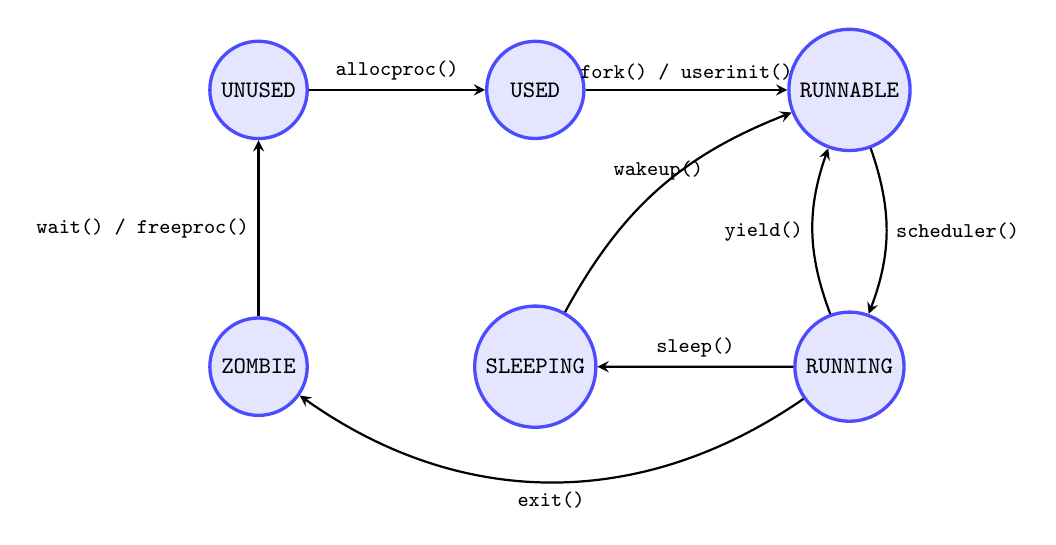
\begin{tikzpicture}[->, >=stealth, node distance=2.2cm, auto,
  state_node/.style={circle, draw=blue!70, fill=blue!10, very thick, minimum size=1.3cm, font=\small\bfseries},
  scale=0.95, every node/.style={transform shape}]

  \node[state_node] (unused) {\texttt{UNUSED}};
  \node[state_node, right of=unused, xshift=1.5cm] (used) {\texttt{USED}};
  \node[state_node, right of=used, xshift=2.0cm] (runnable) {\texttt{RUNNABLE}};
  \node[state_node, below of=runnable, yshift=-1.5cm] (running) {\texttt{RUNNING}};
  \node[state_node, left of=running, xshift=-2.0cm] (sleeping) {\texttt{SLEEPING}};
  \node[state_node, below of=unused, yshift=-1.5cm] (zombie) {\texttt{ZOMBIE}};

  % Transitions
  \path[thick]
    (unused) edge node[above, font=\footnotesize] {\texttt{allocproc()}} (used)
    (used) edge node[above, font=\footnotesize] {\texttt{fork() / userinit()}} (runnable)
    (runnable) edge[bend left=20] node[right, font=\footnotesize] {\texttt{scheduler()}} (running)
    (running) edge[bend left=20] node[left, font=\footnotesize] {\texttt{yield()}} (runnable)
    (running) edge node[above, font=\footnotesize] {\texttt{sleep()}} (sleeping)
    (sleeping) edge[bend left=20] node[above, font=\footnotesize] {\texttt{wakeup()}} (runnable)
    (running) edge[bend left=35] node[below, font=\footnotesize] {\texttt{exit()}} (zombie)
    (zombie) edge node[left, font=\footnotesize] {\texttt{wait() / freeproc()}} (unused);
\end{tikzpicture}
\end{center}

\paragraph{Quy tắc đồng bộ khóa \texttt{p->lock}:}
Bất kỳ thao tác đọc hoặc ghi nào lên trường \texttt{state} đều bắt buộc phải giữ spinlock \texttt{p->lock}. Lý do:
\begin{itemize}
    \item Trên hệ thống đa CPU, hàm \texttt{scheduler()} trên từng CPU liên tục duyệt qua bảng \texttt{proc[]} để tìm tiến trình ở trạng thái \texttt{RUNNABLE}. Nếu không có \texttt{p->lock}, hai CPU có thể cùng lúc thấy một tiến trình là \texttt{RUNNABLE} và cùng chọn nó vào chạy, dẫn đến xung đột bộ nhớ nghiêm trọng.
    \item Việc chuyển trạng thái sang \texttt{SLEEPING} hoặc \texttt{ZOMBIE} đi kèm với các thao tác chuyển luồng điều khiển; khóa \texttt{p->lock} bảo vệ tính nguyên tử của cả chuỗi thao tác này.
\end{itemize}

\subsubsection{Trường \texttt{context} và Chuyển ngữ cảnh (Context Switching)}
Cấu trúc \texttt{struct context} (\texttt{kernel/proc.h}) chứa $14$ trường thanh ghi 64-bit của kiến trúc RISC-V:
\begin{itemize}
    \item \texttt{ra}: Return Address (địa chỉ lệnh sẽ quay về khi kết thúc hàm).
    \item \texttt{sp}: Stack Pointer (con trỏ đỉnh ngăn xếp của kernel thread).
    \item \texttt{s0} -- \texttt{s11}: Callee-saved registers (các thanh ghi mà hàm được gọi có nghĩa vụ bảo toàn giá trị cho hàm gọi nó theo quy ước gọi hàm của RISC-V ABI).
\end{itemize}

\needspace{12\baselineskip}
\paragraph{Phân biệt \texttt{struct context} và \texttt{struct trapframe}:}\leavevmode
\begin{table}[H]
\centering
\begin{tabularx}{\textwidth}{|l|X|X|}
\hline
\textbf{Tiêu chí} & \textbf{\texttt{struct context}} & \textbf{\texttt{struct trapframe}} \\ \hline
\textbf{Không gian lưu} & Kernel context & User context \\ \hline
\textbf{Mục đích} & Chuyển đổi giữa 2 \textbf{kernel thread} (giữa tiến trình và vòng lặp \texttt{scheduler()}). & Lưu trữ trạng thái của \textbf{chương trình người dùng} khi xảy ra ngắt/ngoại lệ/syscall. \\ \hline
\textbf{Tập thanh ghi lưu} & Chỉ lưu các thanh ghi \textbf{callee-saved} (\texttt{ra}, \texttt{sp}, \texttt{s0}--\texttt{s11}). Các thanh ghi caller-saved tự động được lưu trên kernel stack nhờ trình biên dịch C. & Lưu \textbf{toàn bộ thanh ghi người dùng} ($32$ thanh ghi RISC-V) vì tiến trình user có thể bị ngắt tại bất kỳ lệnh assembly nào. \\ \hline
\textbf{Cơ chế thực hiện} & Hàm hợp ngữ \texttt{swtch()} (\texttt{kernel/swtch.S}) được gọi tường minh từ mã C trong kernel. & Mã hợp ngữ \texttt{uservec} / \texttt{userret} trong \texttt{kernel/trampoline.S} khi chuyển chế độ U-mode $\leftrightarrow$ S-mode. \\ \hline
\textbf{Vị trí lưu trữ} & Nằm trực tiếp bên trong \texttt{struct proc} của tiến trình hoặc \texttt{struct cpu} của CPU. & Một trang bộ nhớ riêng (\texttt{PGSIZE = 4KB}) ánh xạ ngay dưới trang trampoline trong không gian địa chỉ tiến trình. \\ \hline
\end{tabularx}
\caption{So sánh giữa \texttt{struct context} và \texttt{struct trapframe}}
\end{table}
